\section{Background and Context}
\label{sec:background}

Behavioral synthesis~\cite{lin:survey-97} is an automated compilation process where a behavioral synthesis tool ~\cite{spark,xpilot,legup}  takes an ESL description, together with a library of hardware resources. Analogous to a regular compiler,
the tool performs the standard lexical and syntax analysis to generate an intermediate representation (IR). The IR is then subjected to a number of
transformations which can be categorized into three phases as shown in Figure~\ref{fig:certification-framework}.

 \begin{enumerate}
\item {\bf Compiler Transformations:} These include typical
  compiler operations, {\em e.g.,} dead-code elimination,
  constant propagation etc. 
\item {\bf Scheduling Transformations:} Scheduling entails
  computing for each operation the clock cycle of its
  execution, accounting for hardware resource constraints
  and control/data dependencies.  Loop pipelining is a component 
  of this phase.
\item {\bf Resource Allocation and Control Synthesis:} This phase
  involves mapping a hardware resource to each operation, allocating
  registers to variables, and generating a controlling finite-state
  machine to implement the schedule.
\end{enumerate}
After the three phases above, the design can be expressed in
RTL which goes through further optimizations. 

\begin{figure}[t!]
\begin{center}
\begin{tabular}{c}
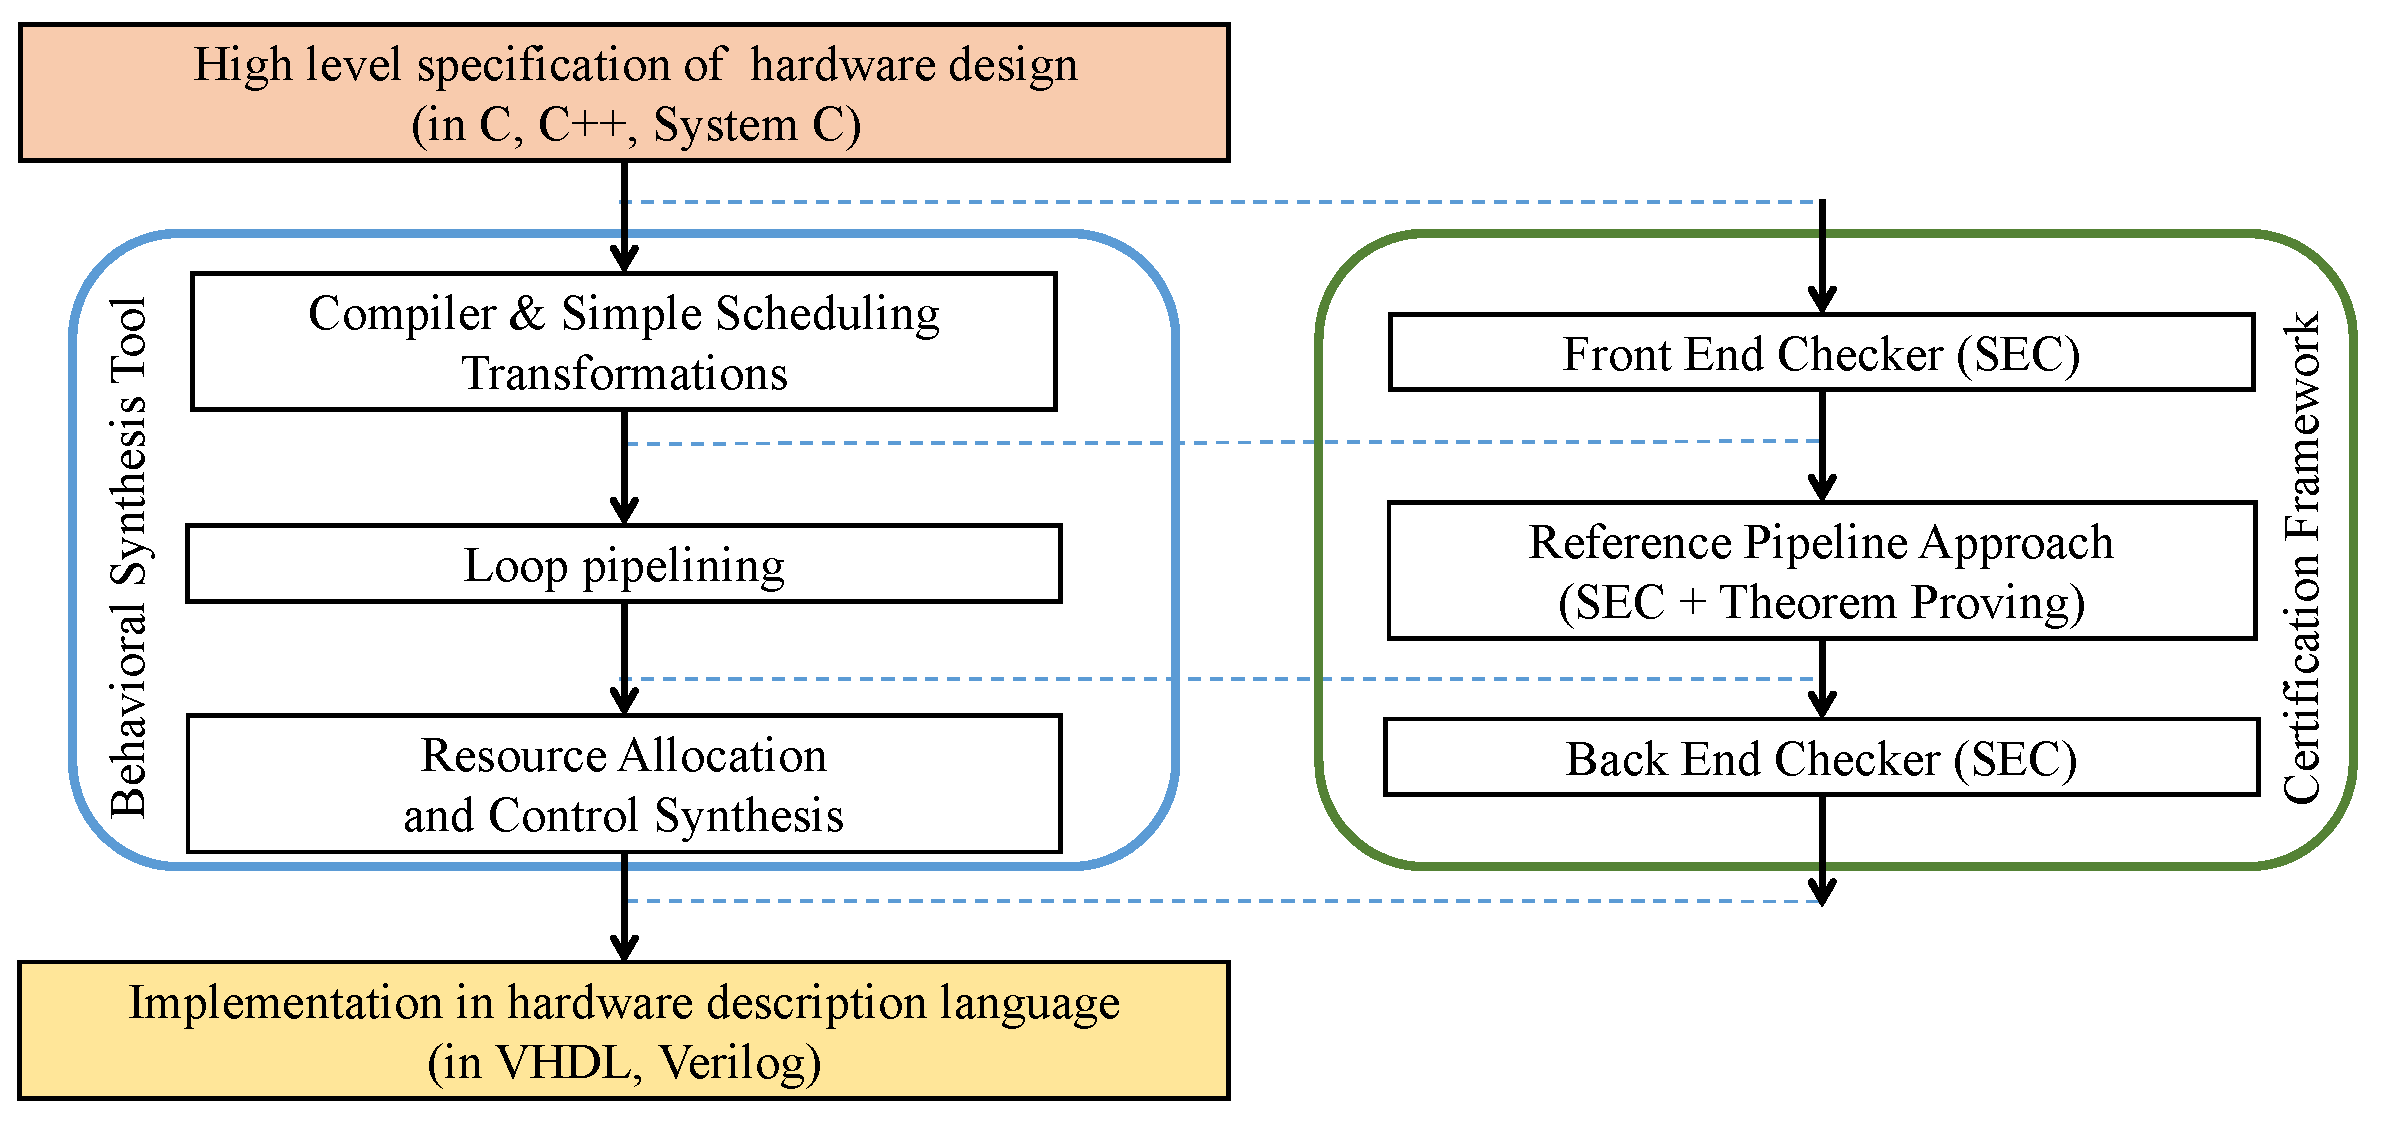
\includegraphics[height=2in]{fig-proposal/certification-framework}
\end{tabular}
\end{center}
\caption{Certification Model for Behaviorally Synthesized Pipelines}
\label{fig:certification-framework}
\end{figure}

There is a large gap in abstraction
between the ESL and RTL descriptions so that there is little
correspondence in internal variables between the two.  Consequently,
direct SEC between the two reduces to cost-prohibitive computation of
input-output equivalence. Applying theorem proving
is also troublesome since extensive manual effort is necessary and
this effort needs to be replicated for each different synthesized
design. It is also infeasible to
directly certify the implementation of the {\em synthesis tool} via
theorem proving.  In addition to being highly complex and thus
potentially requiring prohibitive effort to formally verify with any
theorem prover, the implementations are typically closed-source and
closely guarded by EDA vendors and thus out of reach of external
automated reasoning communities.

Some solutions have been proposed to divide the overall certification problem into manageable portions.
An SEC technique has been tested on industrial strength designs which can compare the RTL 
with the intermediate representation (IR) generated by the tools after the high-level (compiler and scheduling)
transformations have been applied~\cite{rhcxy:atva-09,hxry:date-10}.  In particular,
operation-to-resource mappings generated by the synthesis
tool provide the requisite correspondence between internal
variables of the IR and RTL. There is another SEC technique that 
can certify that the input ESL indeed corresponds to the extracted 
IR produced after the compiler and scheduling transformations applied in the
first two phases of synthesis~\cite{zhenkun:iccd-13}. This technique
can only compare two IRs that are structurally close.  If a
transformation significantly transforms the structure of an IR then
the heuristics for detecting corresponding variables between the two
IRs will not succeed, causing equivalence checking to fail.
Unfortunately, loop pipelining falls in the category of
transformations that significantly changes the structure of the IR.
It is a quintessential transformation that changes the control/data
flow and introduces additional control structures (%\eg, 
to eliminate. Thus a specialized approach is warranted for
handling its certification.

Hao {\em et al.} proposed a pipeline generation algorithm using feedback (like pipeline interval) from the synthesis tool~\cite{hrx:dac-12}. 
They show that to verify the correspondence between sequential CCDFG and pipelined RTL, it is sufficient to perform the following three steps. 
\begin{enumerate} 
\item Check that the algorithm can generate a pipeline reference model for the parameters reported by synthesis.
\item Use SEC to compare the pipeline reference model with the synthesized RTL.
\item Prove the correctness of the algorithm. 
\end{enumerate}
The pipelining algorithm is simpler than that used by the synthesis tool because the synthesis tool uses advanced heuristics to determine the pipeline parameters (such as how many iterations to pipeline, when to introduce stalls etc.), while this pipelining algorithm only uses those parameters to generate a reference model. The algorithm is shown to be scalable but it is not certified. 

Our first approach was to certify this implementation as it is using theorem proving. 
But, our experience was that it is a difficult approach, one that we need not endure. 
In general, in order to certify such an arbitrary implementation,
one has to either (1)~restructure the implementation into
one that is more disciplined, and prove the equivalence
between the two, or (2)~come up with very complex
invariants that essentially comprehend how invariants from
each individual piece are conflated together in the
implementation.  Both approaches require extensive human
interaction, resulting in the proverbial euphemism of proofs
of programs being orders of magnitude more complex than the
programs themselves~\cite{liu}.

In our work, however, we can ``get away'' without verifying
the specific implementation while still being able to
certify the design generated by behavioral synthesis without
loss of fidelity. The key observation, as above, is that it
is sufficient to develop {\em any} certifiable algorithm
that generates a pipelined CCDFG from a sequential
implementation which can be effectively applied with SEC.
In particular, any certifiable algorithm that has the same
input-output characteristic as the proposed algorithm
is sufficient.  Thus, our work is on identifying
certifiable primitives and invariants of a loop pipelining
transformation and developing a pipeline generation
algorithm using those primitives, achieving the dual goal of
mechanical reasoning of the algorithm and amenability of the
resulting reference model to SEC.

Note that our framework is independent of the inner workings of a specific tool, 
and can be applied to certify designs synthesized by different tools from a broad 
class of ESL descriptions. Also, the approach produces a certified reference flow, 
which makes explicit generic invariants that must be preserved by different transformations. 







